\scanpage{109}
\mspage{108}

5): Soit $\underline{C}$ une $\unsure{\otimes|\Omega}$-catégorie tensorielle, \deleted{Pour} munie d'un foncteur fibre sur $k$ \inserted{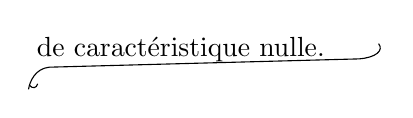
\begin{tikzpicture}[baseline=-.2ex,x=1em,y=1em]
\node[anchor=base west] at (0,.5) {de caractéristique nulle.};
\draw (.05,-.7) .. controls (.1,-.4) and (.3,.05) .. (.8,.1) -- (12,.4) .. controls (12.6,.45) and (12.9,.7) .. (12.7,.95);
\draw (.08,-.55) .. controls (.2,-.7) and (.35,-.65) .. (.38,-.5);
\end{tikzpicture}} A prouver que, pour que le groupe de Galois $G$ correspondant soit profini, il faut et il suffit que pour tout objet $M$ de $\underline{C}$, la $\otimes$-catégorie engendrée soit semi-simple et n'ait qu'un nombre fini d'objects simples non isomorphes. Si $\underline{C}$ est quelconque, la sous-catégorie pleine \deleted{de} $\underline{C}_o$ de $\underline{C}$ qui correspond au pro-groupe quotient de $G$ formé des $\inserted{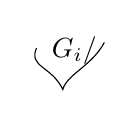
\begin{tikzpicture}[baseline=-.2ex,x=1em,y=1em]
\node[anchor=base west] at (0,.5) {$G_i\handwritten{/}$};
\draw (-.2,.85) .. controls (-.5,.15) and (.35,.2) .. (.75,-.65) .. controls (.9,-.1) and (1.8,.2) .. (2.25,1.05);
\end{tikzpicture}}G_i^o$ (où $G=\underset{\handwritten{\longleftarrow}}{\lim}G_i$, et $G_i^o$ est la composante neutre de $G_i$) est\rlap{\raisebox{-.9ex}{\tikz[x=1em,y=1em]{\fill (0,0)--(.12,.02)--(.08,.13)--cycle;\fill (.09,.2)--(.16,.28)--(.1,.36)--cycle;}}} formée exactement des objets $M$ ayant la propriété précédente.

Il serait intéressant de trouver des énoncés correspondants en caractéristique quelconque.

6) La notion de polarisation d'un motif sur un corps (elle-même déduite de celle de polarisation d'une variété algébrique) donne une structure supplémentaire remarquable dans la catégorie des motifs: si $M$ est un motif de poids $n$, on sait parmi les formes symétriques ($n$ pair) resp. alternées ($n$ impair) $M\otimes M\handwritten{\rightharpoonup} T(n)$ (où $T$ est le motif de Tate) distinguer celles qui sont ``définies positives'' ou encore des \handwritten{``}po$\mathbb{l}$arisations\handwritten{''}. Cette notion se reflête par exemple par des structures supplémentaires sur les groupesde Galois motiviques. Il y a lieu de faire une étude axiomatique abstraite d'une telle notion de polarisation sur une $\otimes$-catégorie générale au dessus d'un \deleted{corps} sous-corps du corps des réels. On pourra en rediscuter à l'occasion.\margin{\tikz[x=1em,y=1em]{\draw (0,0).. controls (.08,.02) and (.16,.14)..(.2,.28);}}

